\section{单粒子态}
我们已经找到了Poincar\'e群所有生成元的的代数关系,可以开始推导单粒子态的表示\footnote{也就是单粒子态是Poincar\'e群的不可约表示,也称为诱导表示。};
回想 \(\left[\mathscr{P}^\nu,\mathscr{P}^\mu\right]=0\)，四动量的对易关系意味着它们有共同的本征态。而且，由于 \(\mathscr{P}^0=\mathscr{H}\)，表明 \(\boldsymbol{p}\) 是一个守恒量。我们首先用 \(p^\mu\) 标记粒子本征态，即。
\begin{equation}\label{4.7}
    \mathscr{P}^\mu\ket{p^\mu,\sigma}=p^\mu\ket{p^\mu,\sigma}
\end{equation}
这里,用 \(p^\mu\) 标记粒子隐含意味着我们已经部分约化了表示矩阵\footnote{例如，具有不同动量的粒子，或正定质量与零质量粒子，不能相互变换}。\(\sigma\) 包括除动量以外的其他指标。
\par
\vspace{2ex}\noindent
考虑粒子在非齐次洛伦兹变换下的变换:
\[U(\Lambda,\;\;a)\ket{p^\mu,\sigma}=?\]
这里，由于 \(U(\Lambda,\;\;a)=U(\Lambda)U(1,\;\;a)\)，因此分为：
\begin{itemize}
    \item 纯时空平移：
    $U(1,\;\;a)\ket{p^\mu,\sigma}=e^{-ip^\mu\;\;a_\mu}\ket{p^\mu,\sigma}$
    此变换是trivial的。
    \item 其次部分的变换:利用计算技巧：$\mathscr{P}^\mu U(\Lambda)\ket{p^\mu,\sigma}=\underbrace{U(\Lambda)U^{-1}(\Lambda)}_{\mathbf{1}}\mathscr{P}^\mu U(\Lambda)\ket{p^\mu,\sigma}
    =\Lambda^\mu_{\;\;\nu}p^\nu U(\Lambda)\ket{p^\mu,\sigma}$
    可以看出 \(U(\Lambda)\ket{p^\mu,\sigma}\) 的本征态 是\(\ket{\Lambda^\mu_{\;\;\nu}p^\nu,\sigma}\),所以：
    \begin{equation}
        U(\Lambda)\ket{p^\mu,\sigma}=\sum_{\bar{\sigma}} C_{ \bar{\sigma}\sigma}(\Lambda,p)\ket{(\Lambda p)^\mu,\bar{\sigma}}
    \end{equation}
\end{itemize}
问题现在归结为：如何找出表示矩阵 \(C_{\sigma\bar{\sigma}}(\Lambda,p)\)的具体形式；考虑\text{Lorentz}变换下的不变量只有$p^2=\eta_{\mu\nu}p^\mu p^\nu$,以及$p^2\geqslant0$时$p^0$的符号；所以我们选择一组标准动量${k^\mu}$\footnote{对于SU(2)，也就是正定质量的粒子，是它们的静止系；对于ISO(2),也就是零质量粒子，不存在静止参考系，所以我们选择那些使得纵向极化消失的坐标系。}
并且任意系中的动量可以通过一个标准\text{boost}得到${k^\mu}$，即：
\begin{equation}
    p^\mu=L^\mu_{\;\;\nu}(p)k^\nu
\end{equation}
所以，动量为$p^\mu$的本征态写为：
\begin{equation}\label{4.10}
    \ket{p^\mu,\sigma}=N(p)U\left\{L(p)\right\}\ket{k^\mu,\sigma}
\end{equation}
用任意\text{Lorentz}变换，作用到(\refeq{4.10})上,得到：
\begin{equation}\label{4.11}
      \begin{aligned}
        U(\Lambda)\ket{p^\mu,\sigma}&=
        N(p)U(\Lambda)U\left\{L(p)\right\}\ket{k^\mu,\sigma}\\
        &=  N(p)U\left\{L(\Lambda p)\right\}\left[U^{-1}\left\{L(\Lambda p)\right\}U(\Lambda)U\left\{L(p)\right\}\right]\ket{k^\mu,\sigma}\\
        &= N(p)U\left\{L(\Lambda p)\right\}U\left\{\underbrace{L^{-1}(\Lambda p)\Lambda L(p)}_{W(\Lambda,p)\text{}}\right\}\ket{k^\mu,\sigma}\\
    \end{aligned}
\end{equation}

\begin{tcolorbox}[colback=white!5,colframe=black!45]
    上面的方程涉及子群 \(W(\Lambda,p) = L^{-1}(p)\Lambda L(k)\)(Wigner小群)。
    \begin{itemize}
        \item \textbf{保持$k^\mu$不变的代数关系}
               $$
                    \begin{aligned}
                        W(\Lambda&,p)= L^{-1}(\Lambda p)\Lambda L(p)\\
                        \Rightarrow &W(\Lambda,p)^\mu_{\;\;\nu}k^\nu= \left[L^{-1}(\Lambda p)\Lambda L(p)\right]^\mu_{\;\;\nu}k^\nu\\
                        &=\left[L^{-1}(\Lambda p)\Lambda \right]^\mu_{\;\;\nu}p^\nu\\
                        &=\left[L^{-1}(\Lambda p)\right]^\mu_{\;\;\nu}\Lambda^\mu_{\;\;\nu}p^\nu\\
                        &=k^\nu
                    \end{aligned}
                    \;\longleftrightarrow \qquad \;
                    \raisebox{-0.5\height}{%
                    \begin{tikzpicture}[>=Stealth, node distance=1.7cm, font=\small]
                    % 节点
                    \node (k) at (0,2) {$k$};
                    \node (p) at (-1.5,0) {$p$};
                    \node (k2) at (1.5,0) {$\Lambda p$};

                    % 圆弧箭头
                    \draw[->, bend right=20] (k) to node[left] {$L(p)$} (p);
                    \draw[->, bend left=20] (k) to node[right] {$L(\Lambda p)$} (k2);
                    \draw[->, bend right=20] (p) to node[below] {$\Lambda$} (k2);

                    \end{tikzpicture}%
                    }
                $$
        $\implies$所以，任意小群作用在标准动量的本质态$\ket{k^\mu,\sigma}$是：
                    $U\left\{W(\Lambda,p)\right\}\ket{k^\mu,a}=\sum_{\bar{\sigma}}D_{\bar{\sigma}\sigma}\left\{W(\Lambda,p)\right\}\ket{k^\mu,\sigma}$
        系数矩阵是小群的一个表示。
        \item \textbf{小群的同态关系}
                $$ D_{\bar{\sigma}\sigma }(\bar{W},W)=\sum_{\bar{\sigma}}D_{\bar{\sigma} \bar{\sigma}'}(\bar{W})D_{\bar{\sigma}'\sigma }(W)$$
    \end{itemize}
\end{tcolorbox}
回到(\refeq{4.11}),利用小群的表示矩阵\footnote{这里的小群就是使得标准动量不变的}：
            \[    \begin{aligned}
                    U(\Lambda)\ket{p^\mu,\sigma}
                    &=N(p)U\left\{L(\Lambda p)\right\}U\left\{W(\Lambda,p)\right\}\ket{k^\mu,\sigma}\\
                    &=\sum_{\bar{\sigma}}D_{\bar{\sigma}\sigma}\left\{W(\Lambda,p)\right\}N(p)U\left\{L(\Lambda p)\right\}\underbrace{\ket{k^\mu,\bar{\sigma}}}_{\text{这里由(\refeq{4.10})变换得到}}\\
                    &=\sum_{\bar{\sigma}}D_{\bar{\sigma}\sigma}\left\{W(\Lambda,p)\right\}N(p)U\left\{L(\Lambda p)\right\}\frac{U^{-1}\left\{L(\Lambda p)\right\}}{N(\Lambda p)}\ket{(\Lambda p)^\mu,\bar{\sigma}}\\
                    &=\frac{N(p)}{N(\Lambda p)}\sum_{\bar{\sigma}}D_{\bar{\sigma}\sigma}\left\{W(\Lambda,p)\right\}\ket{(\Lambda p)^\mu,\bar{\sigma}}
            \end{aligned}
            \]
    归一化系数的选择:$$N(p)=\sqrt{\frac{k^0}{p^0}}$$

$\implies$最终得到：
    \begin{equation}
        U(\Lambda)\ket{p^\mu,\sigma}=\frac{N(p)}{N(\Lambda p)}\sum_{\bar{\sigma}}D_{\bar{\sigma}\sigma}\underbrace{\left\{W(\Lambda,p)\right\}}_{\text{讨论小群的种类参考}\autoref{1}}\ket{(\Lambda p)^\mu,\bar{\sigma}}
    \end{equation}

                \usetikzlibrary{arrows.meta}
                \begin{figure}[htbp]
                \centering
                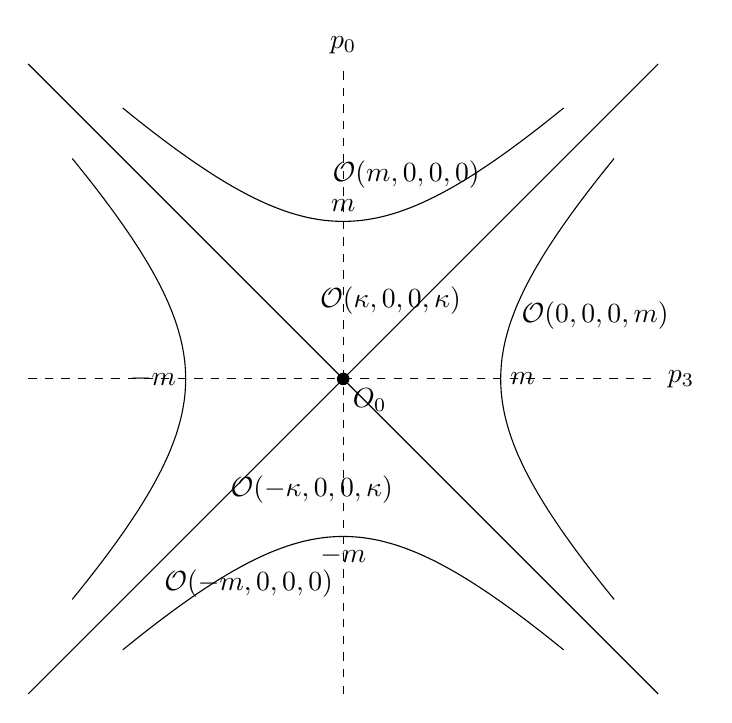
\begin{tikzpicture}[scale=2]
                % ===== 坐标轴 =====
                \draw[dashed] (-2,0) -- (2,0) node[right] {$p_3$};
                \draw[dashed] (0,-2) -- (0,2) node[above] {$p_0$};

                % 原点
                \fill (0,0) circle (0.04) node[below right] {$O_0$};

                % ===== 光锥 =====
                \draw (-2,-2) -- (2,2);
                \draw (-2,2) -- (2,-2);

                % ===== 质量壳：p_0^2 - p_3^2 = m^2 =====
                \draw plot[domain=-1.4:1.4,smooth,variable=\x]
                ({\x},{sqrt(\x*\x+1)});
                \draw plot[domain=-1.4:1.4,smooth,variable=\x]
                ({\x},{-sqrt(\x*\x+1)});

                % ===== 空间样轨道：p_3^2 - p_0^2 = m^2 =====
                \draw plot[domain=-1.4:1.4,smooth,variable=\x]
                ({sqrt(\x*\x+1)},{\x});
                \draw plot[domain=-1.4:1.4,smooth,variable=\x]
                ({-sqrt(\x*\x+1)},{\x});

                % ===== 标注 m, -m =====
                \node[above] at (0,1) {$m$};
                \node[below] at (0,-1) {$-m$};
                \node[right] at (1,0) {$m$};
                \node[left] at (-1,0) {$-m$};

                % ===== 轨道标记 =====
                \node at (0.4,1.3) {$\mathcal O(m,0,0,0)$};
                \node at (-0.6,-1.3) {$\mathcal O(-m,0,0,0)$};

                \node at (1.6,0.4) {$\mathcal O(0,0,0,m)$};

                \node at (0.3,0.5) {$\mathcal O(\kappa,0,0,\kappa)$};
                \node at (-0.2,-0.7) {$\mathcal O(-\kappa,0,0,\kappa)$};

                \end{tikzpicture}
                \caption{Wigner粒子分类的轨道图}
                \label{1}
                \end{figure}
\begin{center}
            \renewcommand{\arraystretch}{1.8}\label{2}
            \begin{tabular}{|c|c|c|c|c|}
            \hline
            类别
            & 四动量条件
            & 图中区域
            & 标准动量 $k^\mu$
            & 小群 $W_k$ \\ \hline

            (I) Massive
            & $p^\mu p_\mu=m^2,\; p^0>0$
            & 光锥内部（上支双曲线）
            & $(m,0,0,0)$
            & $SO(3)\simeq SU(2)$ \\ \hline

            (II) Massless
            & $p^\mu p_\mu=0,\; p^0>0$
            & 光锥本身
            & $(\kappa,0,0,\kappa)$
            & $ISO(2)$ \\ \hline

            (III) Tachyonic
            & $p^\mu p_\mu=-m^2$
            & 光锥外部（左右双曲线）
            & $(0,0,0,m)$
            & $SO(2,1)$ \\ \hline

            (IV) Trivial
            & $p^\mu=0$
            & 原点
            & $(0,0,0,0)$
            & 全洛伦兹群 \\ \hline

            \end{tabular}
\end{center}
\topictitle{***}\label{total_lorentz_group}
深入探讨具体的小群之前，需要说明Wigner 小群严格来说是定义在 Poincaré 群中的.

Poincaré 群的元素通常记为二元组 $(\Lambda, a)$，其中 $\Lambda$ 是齐次 Lorentz 变换，$a$ 是时空平移。当该群算符作用在四维动量本征态 $|p, \sigma\rangle$ 上时：
\begin{itemize}
    \item \textbf{纯平移 $a$ 只提供相位}：$U(1, a)|p, \sigma\rangle = e^{-ip \cdot a}|p, \sigma\rangle$
    \item \textbf{Lorentz 变换改变动量}：$p \mapsto \Lambda p$
\end{itemize}
\vspace{2ex}
Wigner 小群\footnote{严格意义上是对某个标准动量 $k$ 的稳定子群}定义为所有不改变该标准动量的 Poincaré 变换的集合：
\begin{equation}
    \boxed{W_k \equiv \{(\Lambda, a) \in \mathbb{P} \mid \Lambda k = k\}}
\end{equation}
请注意，在这个限制条件中\textbf{只出现了 $\Lambda k = k$}。这是因为时空平移 $a$ 根本不改变动量的本征值（它只改变相位）。这意味着，对于\emph{任意}的时空平移 $a$，元素 $(\mathbb{I}, a)$ 都天然属于这个稳定子群。
\vspace{2ex}
\\
因此，这个真正的稳定子群 $W_k$ 在代数结构上表现为半直积：
\begin{equation}
    \boxed{W_k \cong \mathbb{R}^{1,3} \rtimes \mathbb{H}_k, \qquad \text{其中} \quad \mathbb{H}_k \equiv \{\Lambda \in SO(1,3)^\uparrow \mid \Lambda k = k\}}
\end{equation}
也就是说：
\begin{tcolorbox}[colback=white!5,colframe=black!45]
    \begin{center}
    \textbf{Poincaré 的小群 $\mathbb{P}_k$ = 全体时空平移 $\mathbb{R}^{1,3}$ + 保持 $k$ 不变的 Lorentz 子群 $\mathbb{H}_k$。}
\end{center}
\end{tcolorbox}
\vspace{2ex}
为什么在后续的物理计算中，只谈论 $\mathbb{H}_k$（如 $SO(3)$ 或 $ISO(2)$）呢？这是因为在构造粒子的物理态时，平移部分 $\mathbb{R}^{1,3}$ 的作用已经被剥离出来，用于给出时空的平面波演化因子 $e^{-ip\cdot x}$。平移操作是平凡的，绝对不会导致粒子内部自旋/极化指标 $\sigma$ 的混合.真正能把态的内部指标 $\sigma$ 混合起来的，只有非平凡的 Lorentz 稳定子 $\mathbb{H}_k$.
\subsection{正定质量粒子\(\dagger\)}\label{sec:massive-particle}
正定质量粒子（$p^2 = m^2 > 0$，$p^0 > 0$）的标准动量是$k
^\mu=(m,0,0,0)$,保持空间旋转不变的小群是三维旋转群$SO(3)$；也就是Wigner 小群是三维旋转群 ；而为了容纳半整数自旋，必须使用其万有覆盖群 $SU(2)$，单粒子态的变换是：
\begin{equation}
U(\Lambda)|p^\mu,\sigma\rangle
= \sqrt{\frac{(\Lambda p)^0}{p^0}}\;\;
\sum_{\bar{\sigma}} D^{(j)}_{\bar{\sigma}\sigma}\{W(\Lambda,p)\}\;\;
|(\Lambda p)^\mu,\bar{\sigma}\rangle
\end{equation}
其中 $W(\Lambda,p) = L^{-1}(\Lambda p)\;\;\Lambda\;\;L(p)$ 是 Wigner 旋转——一个纯粹的三维空间旋转，而 $D^{(j)}_{\bar{\sigma}\sigma}$ 是 $SU(2)$ 的 $(2j+1)$ 维不可约表示矩阵。因此，构造正定质量粒子态的全部问题归结为：\textbf{找出 $SU(2)$ 的所有有限维不可约表示}。下面利用 Lie 代数方法系统地完成这一任务。
\topictitle{$SU(2)$代数}
$SU(2)$ 的 Lie 代数由三个生成元 $J_1, J_2, J_3$ 构成，满足
\begin{equation}
[J_i, J_j] = i\epsilon_{ijk}\;\;J_k
\end{equation}
其中$SU(2)$包含一个Casimir算符$\pmb{J}^2$，它与所有生成元对易，以及cartan算符$J_3$，它与 $J_1, J_2$ ;且它们是对易的；
\begin{equation}
    [\pmb{J}^2,J_3]=0
\end{equation}
这是重要的，它们张开了一个完备的Hilbert空间，可以标记本征态为$\ket{a,b}$,有本征关系：
\begin{subequations}
    \begin{align}
        &\pmb{J}^2\ket{b,m}=a\ket{b,m}\\
        &J_3\ket{b,m}=m\ket{b,m}
    \end{align}
\end{subequations}
利用$SU(2)$,可以定义一组新的算符：
\begin{equation}
J_{\pm} = J_1 \pm iJ_2
\end{equation}
这组算符满足：
\begin{equation}
[\pmb{J}^2, J_{\pm}]=0\;\;,\qquad
[J_3, J_{\pm}] = \pm J_{\pm}\;\;,\qquad
[J_+, J_-] = 2J_3
\end{equation}
\par
考虑代数关系：
\begin{equation}
    \begin{aligned}
        J_3\;\;J_\pm\ket{b,m}=&\left(J_\pm J_3\pm J_\pm\right)\ket{b,m}\\
        &= (m \pm 1)\;\;J_\pm\ket{b,m}
    \end{aligned}
\end{equation}
可以看到,$J_{\pm}\Ket{b,m}$也是$J_3$的本征态。本征值被提升或降低了1。可以得到代数关系：
\begin{equation}
    J_\pm\ket{b,m} =constant \ket{b,m \pm 1}
\end{equation}
所以算符$J_{\pm}$被称为升降算符。在$SU(2)$的有限维\footnote{具体表现在Hilbert空间中的范数正定}表示中，m应该是一个有限的值，应当有上界和下界,我们约定上界为$m_{max}$下界为$b_{min}$,可以断定代数关系：
\begin{subequations}
    \begin{align}
        &J_+\ket{b,m_{max}}=0\\
        &J_-\ket{b,m_{min}}=0
    \end{align}
\end{subequations}
对第一式作用$J_-$，对第二式作用$J_+$；可以得到：
\begin{equation}
    \begin{aligned}
    0=&J_-\;\;J_+\ket{b,m_{max}}\\
    =& \left(\pmb{J}^2 - J_3^2 - J_3\right)\ket{b,m_{max}}\\  
    =& \left(a - m_{max}^2 - m_{max}\right)\ket{b,m_{max}}  
    \end{aligned}
    \\
    \begin{aligned}
        0=&J_+\;\;J_-\ket{b,m_{min}}\\
        =& \left(\pmb{J}^2 - J_3^2 +J_3\right)\ket{b,m_{min}}\\  
        =& \left(a - m_{min}^2 + m_{min}\right)\ket{b,m_{min}}  
    \end{aligned}
\end{equation}
解出$a$，得到；
\[\begin{aligned}
    &a=m_{max}^2 + m_{max}\\
    &a=m_{min}^2 - m_{min}
\end{aligned}\]
为了使是一个确定的值，必须满足$m_{max}^2 + m_{max} = m_{min}^2 - m_{min}$，成立的条件(同时将b重新约定为j)是
\begin{equation}
    m_{max} = -m_{min} \equiv j
\end{equation}
因此，$J_3$ (同时将m重新约定为$\sigma$)的本征值序列为 
\begin{equation}
    \sigma=j, j-1, j-2, \ldots, -j+1, -j。
\end{equation}
由于 $m_{max} - m_{min} = 2j$ 必须是非负整数，得到 ：
\begin{equation}
    j = 0, \frac{1}{2}, 1, \frac{3}{2}, \ldots
\end{equation}
j的取值代表了$SU(2)$的有限维表示：
\begin{align}
& j = 0,   && \sigma = 0,                        && j(j+1) = 0 \nonumber \\
& j = 1/2, && \sigma = 1/2, -1/2,                && j(j+1) = 3/4 \nonumber \\
& j = 1,   && \sigma = 1, 0, -1,                 && j(j+1) = 2 \nonumber \\
& j = 3/2, && \sigma = 3/2, 1/2, -1/2, -3/2, \quad && j(j+1) = 15/4 \nonumber \\
& \dots    &&                               && 
\end{align}
在讨论$SU(2)$的低维表示前，还需要找出$J_\pm$的本征值，通过计算可以得到：
\begin{equation}
    \begin{aligned}
        \braket{j,\sigma|J_-J_+|j,\sigma}=&\braket{j,\sigma|\pmb{J}^2 - J_3^2 - J_3|j,\sigma}\\
        &= j(j+1) - \sigma^2 - \sigma
    \end{aligned}
\end{equation}
可以看出$J_+$和$J_-$的本征值为：    
\begin{equation}
    J_{\pm}|j,\sigma\rangle = \sqrt{(j \mp \sigma)(j \pm \sigma + 1)}\;|j,\sigma \pm 1\rangle
\end{equation}
\topictitle{低维不可约表示}
$\mathbf{j=0}$ 表示空间维度为 $1$。是平凡表示。
\vspace{2ex}

\noindent
$\mathbf{j=1/2}$ 表示空间维度为 $2$。$J_3$ 的本征值为 $\pm 1/2$。生成元为 $2\times 2$ 矩阵
\begin{equation}
    J_3=\frac{1}{2}
    \begin{bmatrix}
        & 1&0\\
        & 0&-1
    \end{bmatrix}
\end{equation}
所以选择对应的本征矢量为：
\begin{equation}
    \ket{\frac{1}{2},\frac{1}{2}}
    =\begin{bmatrix}
        1 \\
        0
    \end{bmatrix},\qquad
    \ket{\frac{1}{2},-\frac{1}{2}}
    =\begin{bmatrix}
        0 \\
        1
    \end{bmatrix}
\end{equation}
利用$J_\pm$和$J_1$,$J_2$,$J_3$之间的关系：
\begin{equation}
    \begin{aligned}
        &J_1=\frac{1}{2}(J_++J_-)\\
        &J_2=\frac{1}{2i}(J_+-J_-)
    \end{aligned}
\end{equation}
所以可以得到$J_1$和$J_2$作用在本征态上的值
\begin{equation}
    \begin{aligned}
    J_1\Ket{\frac{1}{2},\frac{1}{2}}
    =&\frac{1}{2}(J_++J_-)\Ket{\frac{1}{2},\frac{1}{2}}\\
    =&\frac{1}{2}\sqrt{(j - \sigma)(j + \sigma + 1)}\ket{\frac{1}{2},-\frac{1}{2}}\\
    =&\frac{1}{2}\ket{\frac{1}{2},-\frac{1}{2}}\\
    \end{aligned}\\
    \begin{aligned}
        J_1\Ket{\frac{1}{2},-\frac{1}{2}}
        =&\frac{1}{2}(J_++J_-)\Ket{\frac{1}{2},-\frac{1}{2}}\\
        =&\frac{1}{2}\sqrt{(j + \sigma)(j - \sigma + 1)}\ket{\frac{1}{2},\frac{1}{2}}\\
        =&\frac{1}{2}\ket{\frac{1}{2},\frac{1}{2}}\\
    \end{aligned}
\end{equation}
以及
\begin{equation}
    \begin{aligned}
        J_2\Ket{\frac{1}{2},\frac{1}{2}}
        =&\frac{1}{2i}(J_+-J_-)\Ket{\frac{1}{2},\frac{1}{2}}\\
        =&-\frac{i}{2}\ket{\frac{1}{2},-\frac{1}{2}}\\
    \end{aligned}\\
    \begin{aligned}
        J_2\Ket{\frac{1}{2},-\frac{1}{2}}
        =&\frac{1}{2i}(J_+-J_-)\Ket{\frac{1}{2},-\frac{1}{2}}\\
        =&\frac{i}{2}\ket{\frac{1}{2},\frac{1}{2}}\\
    \end{aligned}
\end{equation}
最终得到$J_1$和$J_2$的矩阵表示为：
\begin{equation}
    J_1=\frac{1}{2}
    \begin{bmatrix}
        & 0&1\\
        & 1&0
    \end{bmatrix},\qquad
    J_2=\frac{1}{2}
    \begin{bmatrix}
        & 0&-i\\
        & i&0
    \end{bmatrix}
\end{equation}
以及Casimir算符$\pmb{J}^2$的矩阵表示为：
\begin{equation}
    \pmb{J}^2=\frac{3}{4}
    \begin{bmatrix}
        & 1&0\\
        & 0&1
    \end{bmatrix}
\end{equation}
\vspace{2ex}
$\mathbf{j=1}$,利用一样的步骤；可以得到
\begin{equation}
    J_3=
    \begin{bmatrix}
        & 1&0&0\\
        & 0&0&0\\
        & 0&-1&0
    \end{bmatrix},\qquad
    J_1=\frac{1}{\sqrt{2}}
    \begin{bmatrix}
        & 0&1&0\\
        & 1&0&1\\
        & 0&1&0
    \end{bmatrix},\qquad
    J_2=\frac{1}{\sqrt{2}}
    \begin{bmatrix}
        & 0&-i&0\\
        & i&0&-i\\
        & 0&i&0
    \end{bmatrix}
\end{equation}
以及casimir算符$\pmb{J}^2$的矩阵表示为：
\begin{equation}
    \pmb{J}^2=
    2
    \begin{bmatrix}
        & 1&0&0\\
        & 0&1&0\\
        & 0&0&1
    \end{bmatrix}
\end{equation}
更高维度的表示可以通过同样的步骤得到。
\topictitle{单粒子态的完整标记}
综合 Wigner 诱导表示框架与 $SU(2)$ 的不可约表示理论，一个正定质量单粒子态由以下量子数完整标记：
\begin{equation}
|p^\mu,\sigma\rangle\;\;,\qquad \sigma = -j,\;\;-j+1,\;\;\ldots,\;\;+j
\end{equation}
\begin{itemize}
\item $p^\mu$：动量
\item $j$：自旋（Poincar\'{e} 群第二个 Casimir 算符 $W_\mu W^\mu$ 的本征值决定），取 $j = 0,\;\;\tfrac{1}{2},\;\;1,\;\;\tfrac{3}{2},\;\;\ldots$
\item $\sigma$：自旋第三分量（$J_3$ 的本征值），取 $2j+1$ 个值。
\end{itemize}

粒子在一般 Lorentz 变换 $\Lambda$ 下的态变换为
\begin{equation}
U(\Lambda)|p,\sigma\rangle
= \sqrt{\frac{(\Lambda p)^0}{p^0}}\;\;
\sum_{\bar{\sigma}=-j}^{+j} D^{(j)}_{\bar{\sigma}\sigma}\{W(\Lambda,p)\}\;\;
|(\Lambda p),\bar{\sigma}\rangle
\end{equation}
其中 $D^{(j)}_{\bar{\sigma}\sigma}$ 是 $SU(2)$ 自旋 $j$  旋转矩阵，$W(\Lambda,p) = L^{-1}(\Lambda p)\;\;\Lambda\;\;L(p)$ 是 Wigner 旋转。关键的物理图像是：粒子的动量在 Lorentz 变换下改变（$\boldsymbol{p}\to\Lambda\boldsymbol{p}$），而自旋态在 $2j+1$ 维内部空间中进行旋转混合——这种混合由 Wigner 旋转通过 $SU(2)$ 表示矩阵来实现。
\subsection{零质量粒子\(\dagger\)}\label{sec:massless-particle}
对于零质量粒子，由于 $p^\mu p_\mu = 0$，不存在静止参考系。沿 $z$ 轴正方向传播的动量作为“标准动量”：
\begin{equation}
    k^\mu = (\kappa, 0, 0, \kappa)^T, \quad (\kappa > 0)
\end{equation}
Wigner 小群的定义是：所有保持标准动量 $k^\mu$ 不变的$W^{\mu}_{\;\;\nu}$ 构成的子群，即满足：
\begin{equation}
    W^{\mu}_{\;\;\nu} k^\nu = k^\mu
\end{equation}
\topictitle{小群的确定}
为了寻找小群的生成元，\footnote{为什么能这么操作，参考\refeq{total_lorentz_group}}考察Lorentz无穷小变换 $W^{\mu}_{\;\;\nu} = \delta^\mu_{\;\;\nu} + \omega^\mu_{\;\;\nu}$。代入小群条件：
\begin{equation}
    (\delta^\mu_{\;\;\nu} + \omega^\mu_{\;\;\nu}) k^\nu = k^\mu \implies \omega^\mu_{\;\;\nu} k^\nu = 0
\end{equation}
将 $k^\nu = (\kappa, 0, 0, \kappa)^T$ 代入上式并对 $\nu$ 求和，我们得到核心约束：
\begin{equation}
    \omega^\mu_{\;\;0} \kappa + \omega^\mu_{\;\;3} \kappa = 0 \implies \omega^\mu_{\;\;0} = -\omega^\mu_{\;\;3}
\end{equation}
小群的参数 $\omega_{\mu\nu}$ 在两个下指标时是严格反对称的（$\omega_{\mu\nu} = -\omega_{\nu\mu}$）。我们使用闵氏度规将上述约束的指标降下来：$\omega^\mu_{\;\;\nu} = \eta^{\mu\rho}\omega_{\rho\nu}$。
\vspace{2ex}
\\
分别考察 $\mu = 1, 2, 3$ 的情况：
\begin{itemize}
    \item 当 $\mu = 1$ 时：$\eta^{11}\omega_{10} = -\eta^{11}\omega_{13} \implies -\omega_{10} = -(-\omega_{13}) \implies \omega_{10} + \omega_{13} = 0$
    \item 当 $\mu = 2$ 时：$\eta^{22}\omega_{20} = -\eta^{22}\omega_{23} \implies -\omega_{20} = -(-\omega_{23}) \implies \omega_{20} + \omega_{23} = 0$
    \item 当 $\mu = 3$ 时：$\eta^{33}\omega_{30} = -\eta^{33}\omega_{33}$。因为反对称性 $\omega_{33}=0$，所以 $\omega_{30}=0$（即不能有 $z$ 方向的 Boost）。
\end{itemize}
\color{blue}此外，约束方程中并未涉及 $\nu = 1, 2$ 的交叉项，因此空间旋转参数 $\mathbf{\omega_{12}}$ 是完全自由的。\normalcolor
\vspace{2ex}
\\
至此，原有的 6 个 Lorentz 自由参数被约束减少了 3 个，只剩下 3 个独立参数：$\omega_{12}$，以及两组相互绑定的参数 $\omega_{01}=\omega_{13}$ 与 $\omega_{02}=\omega_{23}$。

\vspace{2ex}
任意无穷小 Lorentz 变换的幺正算符可以展开为生成元 $\mathscr{J}^{\mu\nu}$ 的组合：
\begin{equation}
    U(\Lambda) = 1 - \frac{i}{2} \omega_{\mu\nu} \mathscr{J}^{\mu\nu}
\end{equation}
其中Rotation生成元和Boost生成元是：
\begin{equation}
    J_i = \frac{1}{2}\epsilon_{ijk}\mathscr{J}^{jk}\qquad
    K_i =\mathscr{J}^{0i}
\end{equation}
具体对应为：$\mathscr{J}^{12} = J_3$，$\mathscr{J}^{23} = J_1$，$\mathscr{J}^{31} = J_2$(其中 $\mathscr{J}^{13} = -J_2$)，$\mathscr{J}^{01} = K_1$，$\mathscr{J}^{02} = K_2$。
\vspace{2ex}
\par
我们将 $\frac{1}{2} \omega_{\mu\nu} \mathscr{J}^{\mu\nu}$ 展开，并代入我们得到的参数约束（$\omega_{13}=\omega_{01}, \omega_{23}=\omega_{02}$）：
\begin{align}
    \frac{1}{2} \omega_{\mu\nu} \mathscr{J}^{\mu\nu} &= \omega_{01}\mathscr{J}^{01} + \omega_{02}\mathscr{J}^{02} + \omega_{12}\mathscr{J}^{12} + \omega_{23}\mathscr{J}^{23} + \omega_{31}\mathscr{J}^{31} \nonumber \\
    &= \omega_{01}K_1 + \omega_{02}K_2 + \omega_{12}J_3 + \omega_{23}J_1 - \omega_{13}J_2 \nonumber \\
    &= \omega_{12}J_3 + \omega_{01}K_1 + \omega_{02}K_2 + \omega_{02}J_1 - \omega_{01}J_2 \nonumber \\
    &= \omega_{12} J_3 + \omega_{01} (K_1 - J_2) + \omega_{02} (K_2 + J_1)
\end{align}\label{massless_lorentz_transf}
此时，物理图像极其清晰，原来互相独立的旋转 $J$ 和推动 $K$，在零质量条件下被迫组合成了新的生成元。我们定义这三个独立的生成元为：
\begin{equation}
    J_3, \quad \Pi_1 \equiv K_1 - J_2, \quad \Pi_2 \equiv K_2 + J_1
\end{equation}
\vspace{2ex}
\topictitle{  $ISO(2)$ 的 Lie 代数}
最后，我们利用已知的 Lorentz 代数来计算这三个新生成元的对易关系。首先计算 $J_3$ 对 $\Pi_1, \Pi_2$ 的作用：
\begin{subequations}
    \begin{align}
    [J_3, \Pi_1] &= [J_3, K_1] - [J_3, J_2] = iK_2 - (-iJ_1) = i(K_2 + J_1) = i\Pi_2 \\
    [J_3, \Pi_2] &= [J_3, K_2] + [J_3, J_1] = -iK_1 + iJ_2 = -i(K_1 - J_2) = -i\Pi_1
\end{align}
\end{subequations}
再计算 $\Pi_1, \Pi_2$ 自身的对易子：
\begin{align}
    [\Pi_1, \Pi_2] &= [K_1 - J_2, K_2 + J_1] \nonumber \\
    &= [K_1, K_2] + [K_1, J_1] - [J_2, K_2] - [J_2, J_1] \nonumber \\
    &= (-iJ_3) + 0 - 0 - (-iJ_3) \nonumber \\
    &= 0
\end{align}
总结得到的代数关系：
\begin{subequations}
    \begin{align}
        & [J_3, \Pi_1] = i\Pi_2 \\
        & [J_3, \Pi_2] = -i\Pi_1 \\
        & [\Pi_1, \Pi_2] = 0
    \end{align}
\end{subequations}
这在数学上同构于二维欧几里得平面的刚体运动群 $ISO(2)$。其中 $\Pi_1, \Pi_2$ 表现为平面上互相独立的“平移”，而 $J_3$ 表现为平面上的“旋转”。
\topictitle{物理的约束}
$ISO(2)$ 的一般不可约表示可以用 $\Pi_1,\Pi_2$ 的本征值 $\pi_1,\pi_2$ 来标记\footnote{这里采用k标记动量，是约定俗称的}
\begin{subequations}
    \begin{align}
        & \Pi_1|k,\pi_1,\pi_2\rangle = \pi_1 |k,\pi_1,\pi_2\rangle \\
        & \Pi_2|k,\pi_1,\pi_2\rangle = \pi_2 |k,\pi_1,\pi_2\rangle
    \end{align}
\end{subequations}
（因为 $[\Pi_1,\Pi_2]=0$，它们可以同时对角化）。\color{blue}但 $[J_3,\Pi_i]$ 的对易关系表明 $J_3$ 会将 $(\pi_1,\pi_2)$ 在二维平面内旋转，而不改变 $\pi_1^2+\pi_2^2$ 的值。因此 $\pi_1^2+\pi_2^2$ 是一个 Casimir 算符.\normalcolor
\vspace{2ex}
\\
若 $\pi_1^2+\pi_2^2 \neq 0$，则 $J_3$ 的谱是连续的——$J_3$ 的作用等价于在以 $\sqrt{\pi_1^2+\pi_2^2}$ 为半径的圆上旋转。这样的表示称为\textbf{连续自旋表示}。自然界中从未观测到此类粒子。因此物理要求
\begin{equation}
\Pi_1 = \Pi_2 = 0
\end{equation}
即``平移''生成元的本征值为零。这将 $ISO(2)$ 的表示约化为其旋转子群 $SO(2)$ 的表示。

在 $\Pi_1 = \Pi_2 = 0$ 的条件下，剩余的生成元仅有 $J_3$。$SO(2)$ 是阿贝尔群，其全部不可约表示都是一维的，由 $J_3$ 的本征值 $\lambda$ 标记：
\begin{equation}
J_3|k,\lambda\rangle = \lambda\;\;|k,\lambda\rangle
\end{equation}
$\lambda$ 称为\textbf{Helcity}——角动量在动量方向上的投影。
\begin{equation}
\lambda = \frac{\pmb{k} \cdot \pmb{p}}{|\pmb{k}|}
\end{equation}
由于使用的是 Lorentz 群的覆盖群 $SL(2,\mathbb{C})$（与 $SU(2)$ 覆盖 $SO(3)$ 的逻辑完全平行），$\lambda$ 可以取半整数值。对于给定的零质量粒子类型（自旋 $j$），螺旋度只取两个值：
\begin{equation}
\lambda = +j \quad \text{或} \quad \lambda = -j
\end{equation}
本征关系是：
\begin{equation}
  J_3|k,\lambda\rangle = \lambda\;\;|k,\lambda\rangle
\end{equation}
这与正定质量粒子具有 $2j+1$ 个自旋投影形成了鲜明对比。
\topictitle{单粒子态的完整标记}
综合以上分析，零质量单粒子态在 Lorentz 算符变成了
\begin{equation}
    U(\Lambda)=e^{iJ_3\omega_{12}}
\end{equation}
 Wigner 诱导表示框架与 $SU(2)$ 的不可约表示理论，零质量单粒子态由以下量子数完整标记：
\begin{equation}
|k^\mu,\lambda\rangle\;\;,\qquad \sigma = -j,+j
\end{equation}
\begin{itemize}
    \item $k^\mu$：动量
    \item $\lambda$；Helicity。由于 Casimir 算符 $W^2$ 失效，  $\lambda$ 成为了标记粒子内部状态的唯一合法量子数（在标准动量下即为 $J_3$ 的本征值）。对于给定的基本粒子，$\lambda$ 只能取固定的离散值.\normalcolor
\end{itemize}
\begin{equation}
U(\Lambda)|\boldsymbol{p},\lambda\rangle
= \sqrt{\frac{(\Lambda p)^0}{p^0}}\;
e^{i\lambda\theta(\Lambda,p)}\;\delta_{\lambda\bar{\lambda}}
|(\Lambda\boldsymbol{p}),\bar{\lambda}\rangle
\end{equation}
其中 $\theta(\Lambda,p)$ 是 Wigner 旋转中绕 $z$ 轴旋转的角度（Wigner 旋转在零质量情况下退化为一个 $SO(2)$ 旋转加上物理上不可观测的 $\Pi$``平移''）。

